\documentclass{book}
\usepackage{amsmath}
\usepackage{amsthm}
\usepackage{amssymb}
\usepackage[utf8]{inputenc}
\usepackage[german]{babel}
\usepackage{tikz}
\usepackage{multicol}
\usepackage{subcaption}

\newtheorem{proposition}{Proposition}[chapter]
\newtheorem{corollary}{Korollar}[chapter]
\newtheorem{theorem}{Theorem}[chapter]
\newtheorem{lemma}{Lemma}[chapter]
\theoremstyle{definition}
\newtheorem{definition}{Definition}[chapter]
\theoremstyle{remark}
\newtheorem{remark}{Anmerkung}[chapter]
\newtheorem{observation}{Beobachtung}[chapter]
\newtheorem{example}{Beispiel}[chapter]

\newcommand{\nats}[0]{\ensuremath{\mathbb{N}}}
\newcommand{\reals}[0]{\ensuremath{\mathbb{R}}}
\newcommand{\discup}[0]{\ensuremath{\mathrel{\dot{\cup}}}}
\newcommand{\simdif}[0]{\ensuremath{\mathrel{\triangle}}}
\newcommand{\join}[0]{\ensuremath{\mathrel{\nabla}}}

\title{Zusammenfassung: Graphen und biologische Netze}
\author{Felix Linker}

\begin{document}

\maketitle

\tableofcontents

\chapter{Grundlegende Definitionen}

\begin{definition}[Graph]
    Ein Graph $ G = (V, E) $ ein Tupel einer endlichen Knotenmenge $ V $ und einer endlichen Kantenmenge $ E \subseteq \{ \{ v, w \} \mid v, w \in V \} $.
\end{definition}

Im folgenden Sei $ G = (V, E) $ ein fixierter Graph.

\begin{definition}
    Seien $ V_1 \subseteq V $, $ E_1 \subseteq E $ und $ G' = (V', E') $ ein Graph.
    Es seien:
    \begin{itemize}
        \item $ G[V_1] = (V_1, E \cap V_1 \times V_1) $ der von $ V_1 $ \textit{induzierte Teilgraph} von $ G $,
        \item $ G \setminus V_1 = G[V \setminus V_1] $ und
        \item $ G \setminus E_1 = (V, E \setminus E_1) $.
        \item $ G \setminus G' = (G \setminus V') \setminus E' $.
        \item $ G \cup G' = (V \cup V', E \cup E') $.
        \item $ G \cap G' = (V \cap V', E \cap E') $.
    \end{itemize}
\end{definition}

\begin{definition}[Grad]
    Der \textit{Grad} $ \deg(v) $ eines Knoten $ v \in V $ ist die Anzahl der mit ihm in Verbindung stehender Knoten, d.h. $ \deg(v) = |\{ w \mid \{ v, w \} \in E \}| $.

    Der \textit{maximale Grad} $ \Delta(G) $ eines Graphen ist $ \max_{v \in V} \deg(v) $.
    Der \textit{minimale Grad} $ \delta(G) $ eines Graphen ist $ \min_{v \in V} \deg(v) $.
\end{definition}

\begin{definition}[Abstand]
    Der \textit{Abstand} zwischen zwei Knoten $ v_1, v_2 \in V $ ist die Länge des kürzesten Pfades zwischen diesen Knoten.
    Existiert kein solcher Pfad, gilt $ d(v_1, v_2) = \infty $.
\end{definition}

\begin{observation}
    $ d : V \times V \rightarrow \nats $ ist eine Metrik:
    \begin{enumerate}
        \item $ d(v_1, v_2) = 0 $
        \item $ d(v_1, v_2) = d(v_2, v_1) $
        \item $ d(v_1, v_3) \leq d(v_1, v_2) + d(v_2, v_3) $
        \item $ 0 \leq d(v_1, v_2) $
    \end{enumerate}
\end{observation}

\begin{definition}[Durchmesser]
    Der \textit{Durchmesser} $ D $ von $ G $ ist definiert als:
    \begin{equation*}
        D = \max_{v_1, v_2 \in V} d(v_1, v_2)
    \end{equation*}

    D.h., der Durchmesser ist die Länge des längsten kürzesten Wegs in einem Graphen.
\end{definition}

\begin{definition}[Verbundenheit]
    $ G $ ist verbunden, falls für alle Knoten $ v_1, v_2 \in V $ gilt, dass $ d(v_1, v_2) < \infty $, d.h. zwischen allen Knoten existiert ein Pfad.
\end{definition}

\begin{definition}[Cut vertex]
    $ v \in V $ ist ein cut vertex, falls $ G \setminus \{ v \} $ mehr Zusammenhangskomponenten als $ G $ hat.
\end{definition}

\begin{definition}[Cutset]
    $ V_1 \subsetneq V $, falls $ G \setminus V_1 $ mehr Zusammenhangskomponenten als $ G $ hat.
\end{definition}

\begin{definition}[$ k $-(vertex-)Verbundenheit]
    $ G $ ist $ k $-(vertex-)verbunden, falls eine Knotenmenge $ K \subseteq V $ mit $ |K| = k $ existiert, sodass $ G \setminus K $ nicht mehr verbunden ist und $ G $ nicht $ k' $-verbunden für $ k' < k $ ist, d.h. jedes cutset hat mindestens $ k $ Elemente.
\end{definition}

\begin{proposition}
    $ G $ ist 2-verbunden gdw. $ G $ ist verbunden und enthält keinen cut vertex.
\end{proposition}

\begin{definition}[Block]
    $ B = (V_B, E_B) \subseteq G $ ist ein Block, falls $ B $ maximal 2-verbunden ist.
\end{definition}

\begin{definition}[Blockgraph]
    $ G_B $ von $ G $, sodass ein Knoten in $ G_B $ einen Block in $ G $ repräsentiert.
    Zwei Blöcke sind in $ G_B $ miteinander verbunden, falls eine Kante zwischen zwei Knoten der Blöcke in $ G $ existiert.
\end{definition}

\begin{proposition}
    Jeder Blockgraph ist ein Baum bzw. Wald.
\end{proposition}

\begin{definition}[End Block]
    Ein Knoten $ v \in V_B $ in einem Blockgraphen $ G_B = (V_B, E_B) $ ist ein end block, falls $ \deg(v) \leq 1 $, d.h. $ v $ ist ein Blatt im Blockgraph.
\end{definition}

\chapter{Algebraische Graphentheorie \& Kreise}

Im folgenden sei $ G = (V = \{ v_1, \dots, v_n \}, E = \{ e_1, \dots, e_m \}) $ ein fixierter, ungerichteter Graph.

\begin{definition}[Inzidenzmatrix]
    Eine Inzidenzmatrix $ I $ ist eine Matrix der Dimension $ n \times m $ mit:
    \begin{multicols}{2}
        Für ungerichtete Graphen:
        \begin{equation*}
            I_{kl} = \begin{cases}
                0, & v_k \notin e_l \\
                1, & v_i \in e_l
            \end{cases}
        \end{equation*}

        \columnbreak

        Für gerichtete Graphen:
        \begin{equation*}
            I_{kl} = \begin{cases}
                1, & e_l = (v_k, v') \\
                0, & v_k \notin e_l \\
                -1, & e_l = (v', v_k)
            \end{cases}
        \end{equation*}
    \end{multicols}

    \textit{(Die Wahl der jeweiligen Konstanten ist dabei Konvention.)}
\end{definition}

\begin{definition}[Inzidenzstruktur]
    Eine Inzidenzstruktur ist ein Tupel $ (p, B, I) $ mit $ I \subseteq p \times B $ und $ p \cap B = \emptyset $.
    \begin{itemize}
        \item $ p $ ist eine Menge von \textit{Punkten}
        \item $ B $ ist eine Menge von \textit{Blöcken}
        \item $ I $ ist eine \textit{Inzidenzmatrix}
    \end{itemize}
\end{definition}

\begin{definition}[Adjanzenzmatrix]
    Eine Adjanzenzmatrix ist eine Matrix $ A \subseteq \{ 0, 1 \}^{n \times m} $ mit
    \begin{equation*}
        A_{kl} = 1 \Leftrightarrow \{ v_k, v_l \} \in E
    \end{equation*}
\end{definition}

\begin{definition}[Gradmatrix/Degreematrix]
    Eine Gradmatrix ist eine Matrix $ D \subseteq \nats^{n \times m} $ mit
    \begin{equation*}
        D_{kl} = \begin{cases}
            deg(v_k), & k = l \\
            0
        \end{cases}
    \end{equation*}
\end{definition}

\begin{definition}[Laplacematrix]
    Seien $ D $ eine Gradmatrix und $ A $ eine Adjanzenzmatrix.
    Die Laplacematrix $ L $ ist definiert als:
    \begin{equation*}
        L = D - A
    \end{equation*}

    Für einen gerichteten Graphen und dessen Inzidenzmatrix $ I $, kann $ L $ alternativ definiert werden als: $ L = I \cdot I^\top $.
\end{definition}

\section{Algebraische Konnektivität}

\begin{definition}[Eigenwertproblem]
    Sei $ M \subseteq \reals^{n \times m} $ und $ E \in Diag(1)^n $ die entsprechende Einheitsmatrix.
    Das \textit{Eigenwertproblem} beschreibt das finden von Skalaren $ \lambda $ und Vektoren $ x $, sodass
    \begin{align*}
        & Ax = \lambda Ex \\
        \equiv \; & (A - \lambda E) x = 0
    \end{align*}

    Die Menge aller Eigenwerte $ \lambda_i $ induziert das \textit{Eigenspektrum}.
\end{definition}

\begin{definition}[Fiedler Wert/Vektor/Algebraische Konnektivität]
    Der Fiedler Wert ist der zweit-kleinste Eigenwert der Laplacematrix (mehrfach vorkommende Eigenwerte werden mehrfach gezählt).
    Der Fiedler Vektor ist der Eigenvektor des Fiedler Werts.

    Der Fiedler Wert ist die \textbf{algebraische Konnektivität} eines Graphen.
\end{definition}

\begin{proposition}
    Die Anzahl der 0-en im Spektrum der Laplacematrix ist gleich der Anzahl der Zusammenhangskomponenten eines Graphen.
\end{proposition}

\begin{corollary}
    Der Fiedler Wert ist 0 gdw. ein Graph ist nicht verbunden.
\end{corollary}

\begin{observation}
    Sei $ n = |V| $, $ D $ der Durchmesser von $ G $ und sei $ G $ $ k $-verbunden.
    Dann gilt, dass die algebraische Konnektivität $ v $ beschränkt ist durch:
    \begin{equation*}
        \frac{4}{nD} \leq v \leq k
    \end{equation*}
\end{observation}

\begin{observation}
    Der Fiedler Vektor eignet sich zur Partitionierung von Graphen.
    Komponenten dieses Vektors beschreiben die algebraische Verbundenheit des entsprechenden Knotens (es wird der Knoten des jeweiligen Index der Laplace-/Adjanzenzmatrix beschrieben).

    Je kleiner der Wert, desto weniger verbunden ist ein Knoten.
    Zerlegt man $ G $ nach Vorzeichen des Fiedler Vektors in zwei Teilgraphen, erhält man zwei ``optimal'' zusammenhängende Komponenten.
\end{observation}

\subsection{Cauchy Interlace Theorem}

\begin{theorem}[Cauchy Interlace Theorem]
    \label{thm:interlace}
    Sei $ M \subseteq \reals^{n \times n} $ eine symmetrische Matrix, d.h. $ M = M^\top $\footnote{%
        Im eigentlich Theorem ist die Matrix definiert auf den komplexen Zahlen und muss lediglich hermitesch sein, d.h. symmetrisch modulo komplexe Konjugation.
        Dies ist hier jedoch nicht von Relevanz.
    }, mit den Eigenwerten $ \lambda_1 \leq \lambda_2 \leq \dots \leq \lambda_n $.
    Des Weiteren sei $ N \subseteq \reals^{n - 1 \times n - 1} $ eine Teilmatrix von $ M $ mit den Eigenwerten $ \mu_1 \leq \mu_2 \leq \dots \leq \mu_{n - 1} $.

    Dann gilt:
    \begin{equation*}
        \lambda_1 \leq \mu_1 \leq \lambda_2 \leq \mu_2 \leq \dots \leq \mu_{n - 1} \leq \lambda_n
    \end{equation*}
    Dies ist die durch das Theorem beschriebene ``interlacing Struktur''.
\end{theorem}

\begin{observation}
    Das Cauchy Interlace Theorem (\ref{thm:interlace}) beschreibt, welche Auswirkungen das Löschen von Knoten auf die Eigenwerte der Laplacematrix und damit Konnektivität des Graphen hat.
\end{observation}

\section{Konnektivität}

\begin{definition}[Unabhängige Pfade]
    Zwei Pfade $ p = x p_1 \dots p_n y $ und $ q = x q_1 \dots q_m y $ sind unabhängig, falls $ p_i \neq q_j $ für $ 1 \leq i \leq n, 1 \leq j \leq n $.
\end{definition}

\begin{proposition}[Charakterisierung von $ k $-Verbundenheit]
    \label{prp:char-k-connected}
    $ G $ ist $ k $-verbunden, falls:
    \begin{enumerate}
        \item Alle $ k - 1 $ großen, induzierten Subgraphen verbunden sind.
        \item Für alle $ v_1, v_2 \in V $, $ k - 1 $-viele, unabhängige Pfade von $ v_1 $ nach $ v_2 $ existieren.
    \end{enumerate}
\end{proposition}

\begin{proposition}[Charakterisierung von 2-Verbundenheit]
    \label{prp:char-2-connected}
    Die Menge aller 2-verbundenen Graphen ist gleich $ \mathcal{V} $.

    $ \mathcal{V} $ sei induktiv definiert durch:
    Sei $ \mathcal{C} $ die Menge aller Kreise.
    $ \mathcal{V} $ ist die kleinste Menge, für die gilt:
    \begin{enumerate}
        \item $ \mathcal{C} \subseteq \mathcal{V} $
        \item Wenn $ G \in \mathcal{V} $ und $ H \notin \mathcal{C} $ ein Pfad mit Endpunkten (und nur Endpunkten) auf $ G $, dann gilt $ G \cup H \in \mathcal{V} $.
    \end{enumerate}
\end{proposition}

\begin{proof}~\par
    \begin{description}
        \item[``$ \subseteq $''] Sei $ G $ 2-verbunden, aber nicht in $ \mathcal{V} $.
        Da $ G $ 2-verbunden, ex. ein Kreis in $ G $.
        Somit ex. ein maximaler, induzierter, echter Subgraph $ H \subsetneq G $ mit $ H \in \mathcal{V} $.

        Da $ G $ verbunden, ex. Kante $ vw \in E $ mit $ w \in H $ und $ v \in G \setminus H $.
        Da $ G $ 2-verbunden, ex. nach Proposition \ref{prp:char-k-connected} ein Pfad zu einem beliebigen anderen Knoten $ w' \in H $, der nicht über $ w $ verläuft.
        Somit existiert in $ G $ aber ein Pfad von $ w $ über $ v $ nach $ w' $.
        Damit aber nach Voraussetzung der Maximalität von $ H $, $ v \in V(H) $.
        Widerspruch.
        \item[``$ \supseteq $''] Offensichtlich.
    \end{description}
\end{proof}

\begin{remark}
    Ähnlich konstruktive Charakterisierungen sind für $ k $-Verbundenheit mit $ 2 < k $ deutlich schwerer.
\end{remark}

\begin{observation}
    Die induktive Definition aus Proposition \ref{prp:char-2-connected} induziert einen Algorithmus zur Generierung 2-verbundener Graphen und Überprüfung, ob ein Graph 2-verbunden ist.
    \begin{enumerate}
        \item Zur Generierung, starte mit einem beliebigen Kreis und füge Pfade hinzu, die selbst kein Kreis sind.
        \item Zur Überprüfung, lösche Pfade aus dem Graphen, die selbst kein Kreis sind, und schau, ob am Ende ein Kreis entsteht.
    \end{enumerate}

    Kreise sind demnach ``atomare'' 2-verbundene Graphen.
\end{observation}

\section{Kreisbasen}

Im Folgenden werden nur zusammenhängende Graphen mit mindestens zwei Knoten betrachtet.
Dadurch lässt sich ein Graph vollständig durch seine Kantenmenge $ E $ beschreiben.
Werden Teilgraphen betrachtet, müssen diese die gleichen Eigenschaften erfüllen.

\begin{remark}
    Die Ergebnisse dieses Abschnitts können auch auf Graphen, die diese Eigenschaften nicht erfüllen, ausgeweitet werden.
    I.~A. bestehen solche Graphen aus Komponenten von 2-zusammenhängenden Graphen, die entweder nicht- oder 1-verbunden sind.
    Solche Komponenten werden \textit{Blöcke} genannt.

    Die Ergebnisse in diesem Abschnitt können dann auf Blöcke angewendet werden.
\end{remark}

\begin{definition}[Charakteristischer Vektor]
    Sei $ F \subseteq E $.
    Der charakteristische Vektor von $ F $, $ \vec{F} \in \{ 0, 1 \}^m $ ist gegeben durch:
    \begin{equation*}
        \vec{F}_i = \begin{cases}
            0, & e_i \notin F \\
            1, & e_i \in F
        \end{cases}
    \end{equation*}
\end{definition}

Im Folgenden werden Mengen von Kanten und charakteristische Vektoren synonym verwendet.
Des Weiteren bezeichne $ \cdot $ die komponentenweise Multiplikation, $ \odot $ die Matrixmultiplikation und $ \oplus $ den XOR Operator.

\begin{proposition}
    \label{prp:xor-odd-even}
    Sei $ A \subseteq E $.
    Es gilt:
    \begin{equation*}
        \bigoplus_{e \in A} e = \begin{cases}
            0, & |A| \mod 2 = 0 \\
            1, & |A| \mod 2 \ne 0
        \end{cases}
    \end{equation*}
\end{proposition}

\begin{proposition}
    Sei $ H $ eine Inzidenzmatrix und $ C \subseteq E $ ein Kreis.
    Dann gilt:
    \begin{equation*}
        H \odot C = 0^m
    \end{equation*}
    oder äquivalent
    \begin{equation*}
        \forall x \in V: (H \odot C)_x = 0 = \bigoplus_{e \in E} (H_{xe} \cdot C_e)
    \end{equation*}
\end{proposition}

\begin{proof}
    Betrachte $ x \in V $.
    Beweis per Fallunterscheidung.
    \begin{enumerate}
        \item Es gelte: $ x $ liegt auf $ C $.

        Dann gilt $ \bigoplus_{e \in E} H_{xe} \cdot C_e = 0 $, da niemals $ H_{xe} = 1 $ ($ x $ ist inzident zu Kante $ e $) und $ C_e = 1 $ (Kante $ e $ ist im Kreis).

        \item Es gelt: $ x $ liegt auf $ C $.

        Dann gibt es genau zwei Kanten auf $ C $, die zu $ x $ inzident sind.
        Somit gilt:
        \begin{align*}
            \bigoplus_{e \in E} H_{xe} &= \big(\bigoplus_{e \in C} H_{xe} \cdot C_e\big) \oplus \big(\bigoplus_{e \in E \setminus C} H_{xe} \cdot C_e\big) \\
            &= (1 \oplus 1 \oplus 0 \oplus 0 \oplus \dots) \oplus (0 \oplus 0 \oplus \dots) \\
            &= 0 \oplus 0 = 0
        \end{align*}
    \end{enumerate}
\end{proof}

\begin{proposition}[Addition von Kreisen]
    \label{prp:circle-add}
    Für zwei Kreise $ C_1, C_2 \subseteq E $ gilt:
    \begin{equation*}
        \vec{C_1} \oplus \vec{C_2} \simeq C_1 \triangle C_2 = (C_1 \cup C_2) \setminus (C_1 \cap C_2)
    \end{equation*}
\end{proposition}

\begin{proposition}
    \label{prp:circle-mult}
    Sei $ F \subseteq E $.
    Es gilt $ H \odot F = 0^m $ gdw. $ F $ ist ein Kreis.
\end{proposition}

\begin{remark}
    Nach Propositionen \ref{prp:circle-add} und \ref{prp:circle-mult} kann jeder Kreis als Kantendisjunkte Summe kleinerer Kreise dargestellt werden.
    Dies motiviert die Definition eines Vektorraums der Kreise.
\end{remark}

\begin{definition}[Kreisraum]
    Sei $ V $ die Menge aller Kreise in $ G $.
    Der \textit{Kreisraum} $ \mathcal{C}(G) $ von $ G $ ist der Vektorraum $ (V, \oplus) $ ohne Skalarmultiplikation, d.h. wenn $ F_1, F_2 \in V $, dann $ F_1 \oplus F_2 \in V $.

    Die Basis dieses Vektorraums wird \textit{Kreisbasis} genannt.
\end{definition}

\begin{definition}[Basis]
    Die \textit{Basis} eines Vektorraums $ \mathcal{V} = (V, \oplus, \odot) $ ist eine Menge $ B = \{ b_1, \dots, b_n \}$ von Vektoren mit:
    \begin{enumerate}
        \item Jeder Vektor $ v \in V $ lässt sich als Linearkombination von Basisvektoren darstellen:
        \begin{equation*}
            v = \bigoplus_{i = 1}^n \lambda_i \cdot b_i
        \end{equation*}
        Die Basis bildet ein \textit{Erzeugendensystem}.

        \item $ B $ ist linear unabhängig und damit insbesondere minimal.
    \end{enumerate}
\end{definition}

\begin{definition}[Lineare Unabhängigkeit]
    Eine Menge von Vektoren $ V = \{ v_1, \dots, v_n \} $ ist linear unabhängig, falls die Gleichung
    \begin{equation*}
        \bigoplus_{i = 1}^m \lambda_i \cdot v_i = 0
    \end{equation*}
    nur die Lösung $ \lambda_1 = \lambda_2 = \dots = 0 $ hat.
\end{definition}

\begin{definition}[Kantenraum]
    Die Menge der Einheitsvektoren $ E $ aus $ \{ 0, 1\}^m $ bildet die Basis das \textit{Kantenraums} $ \mathcal{E}(G) $, der alle Teilgraphen von $ G $ enthält.
\end{definition}

\begin{proposition}
    Es gilt $ \mathcal{C}(G) $ ist ein Unterraum von $ \mathcal{E}(G) $, d.h. insbesondere $ \dim \mathcal{C}(G) \leq \dim \mathcal{E}(G) = m $.
\end{proposition}

\section{Schnitte}

\begin{definition}[Schnitt]
    Eine Menge $ K \subseteq E $ ist ein Schnitt, falls $ (V, E \setminus K) $ nicht zusammenhängend ist.
\end{definition}

\begin{definition}[Elementarer Schnitt]
    Der elementare Schnitt für einen Knoten $ v \in V $ ist definiert als $ K_v = \{ e \in E \mid v \in e \} $.
\end{definition}

\begin{definition}[Cut]
    Sei $ A \subsetneq V $, $ A \ne \emptyset $.
    $ Cut(A) = \{ e \in E \mid e \cap A \ne \emptyset, e \cap (V \setminus A) \ne \emptyset \} $, d.h. die Menge der Kanten, die einen Endpunkt in $ A $ und einen Endpunkt in $ V \setminus A $ haben.
\end{definition}

\begin{proposition}
    Sei $ A \subsetneq V $, $ A \ne \emptyset $.
    Es gelten jeweils:
    \begin{enumerate}
        \item $ Cut(A) = Cut(V \setminus A) $ und
        \item $ Cut(A) = \bigoplus_{v \in A} K_v $.
    \end{enumerate}
\end{proposition}

\begin{proof}
    \begin{enumerate}
        \item Offensichtlich.
        \item Betrachte $ e \in E $ mit $ e \subseteq A $.
        Dann ex. genau zwei elementare Schnitte von Knoten aus $ A $, die $ e $ enthalten.
        Somit $ (\bigoplus_{v \in A} K_v)_e = 0 $.

        Betrachte nun $ e \in E $ mit $ e \cap A = \emptyset $.
        Dann ex. kein elementarer Schnitt, der $ e $ enthält, somit ist die entsprechende Vektor-Komponente auch hier gleich $ 0 $.

        Angenommen $ e \in E $ mit $ e \cap A \ne \emptyset $, aber $ e \not \subseteq A $.
        Dann ex. genau ein elementarer Schnitt von Knoten aus $ A $, der $ e $ enthält.
        Somit ist die entsprechende Vektor-Komponente gleich $ 1 $.
    \end{enumerate}
\end{proof}

\begin{corollary}
    Es gilt:
    \begin{equation*}
        Cut(A) \oplus Cut(V \setminus A) = 0 = \bigoplus_{v \in V} K_v
    \end{equation*}

    Somit ist die Menge aller elementaren Schnitte linear abhängig.
\end{corollary}

\begin{definition}[Schnittraum]
    Sei $ V $ die Menge aller Schnitte.
    Der \textit{Schnittraum} $ \mathcal{K}(G) $ von $ G $ ist der Vektorraum $ (V, \oplus) $ ohne Skalarmultiplikation.
\end{definition}

\begin{proposition}
    Seien $ K, C \subseteq E $ ein Schnitt und ein Kreis.
    Dann gilt
    \begin{equation*}
        \bigoplus_{e \in E} K_e \cdot C_e = \bigoplus_{e \in K \cap C} 1 = 0
    \end{equation*}
\end{proposition}

\begin{proof}
    Es genügt, zu zeigen, dass $ |K \cap C| \mod 2 = 0 $ (vgl. Prop. \ref{prp:xor-odd-even}).
    Da $ K $ ein Schnitt ist, muss $ C \setminus K $ eine Menge von Pfaden sein.
    Eine Menge von Pfaden könnte aber nicht durch eine ungerade Anzahl von Kanten zu einem Kreis verbunden werden, somit muss $ |K \cap C| $ gerade sein.
\end{proof}

\begin{proposition}
    Es gilt:
    \begin{equation*}
        \dim \mathcal{K}(G) + \dim \mathcal{C}(G) = |E| = \dim \mathcal{E}(G)
    \end{equation*}
\end{proposition}

\begin{remark}
    Schnitte und Kreise sind also orthogonal.
\end{remark}

\begin{definition}[Spannbaum]
    Der \textit{Spannbaum} eines zusammenhängen Graphen ist der Teilgraph $ W \subseteq G $, der ein zusammenhängender Baum ist und jeden Knoten von $ G $ enthält.
\end{definition}

\begin{remark}
    Ein Baum mit mit $ |V| $ Knoten, enthält $ |V| - 1 $ Kanten.
\end{remark}

\begin{definition}[Erweiterter Cut]
    Sei $ T $ ein Spannbaum von $ G $ und $ e $ eine Kante in $ T $.
    Dann ist $ Cut(T, e) $ die Menge aller Kanten in $ G $, die die Zusammenhangskomponenten verbinden, die sich durch entfernen von $ e $ in $ T $ ergeben.
\end{definition}

\begin{proposition}
    \label{prp:cuts-independent}
    Für einen fixierten Spannbaum $ T $ ist die Menge aller Schnitte $ Cut(T, e) $, $ e \in E(T) $ linear unabhängig.
\end{proposition}

\begin{proof}
    Seien $ T = (V_T, E_T) $, $ e, e' \in E_T $.
    Es gilt, dass $ e \in Cut(T, e') $ gdw. $ e = e' $.
    Somit gilt insbesondere für alle Folgen von Knoten $ e_1, e_2, \dots \in E $ mit $ e_i \ne e $: $ Cut(T, e_1)_e = 0 $, $ Cut(T, e_2)_e = 0 $, etc., und damit $ e \notin Cut(T, e_1) \oplus Cut(T, e_2) \oplus \dots $.
\end{proof}

\begin{proposition}
    Jeder Schnitt kann als eine Summe aus Schnitten $ \{ Cut(T, e) \mid e \in T \} $ für einen fixierten Spannbaum $ T $ dargestellt werden.
\end{proposition}

\begin{proposition}
    \label{prp:dim-bases}
    Beachte, dass $ |\{ Cut(T, e) \mid e \in T \}| = |V| - 1 $.
    Somit
    \begin{equation*}
        \dim \mathcal{K}(G) = |V| - 1
    \end{equation*}
    und daher
    \begin{equation*}
        \dim \mathcal{C}(G) = |E| - \dim \mathcal{K}(G) = |E| - |V| + 1
    \end{equation*}
\end{proposition}

\begin{definition}[Cyc]
    Sei $ T = (V_T, E_T) $ ein Spannbaum und $ e \notin E_T $.
    $ Cyc(T, e) $ sei der eindeutig bestimmte Kreis in $ (V_T, E_T \cup \{ e \}) $.
\end{definition}

\begin{proposition}
    \label{prp:cyc-independent}
    Sei $ T = (V_T, E_T) $ ein Spannbaum.
    Die Menge $ \{ Cyc(T, e) \mid e \in E \setminus E_T \} $ ist linear unabhängig.
\end{proposition}

\begin{proof}
    Dieser Beweis kann analog zum Beweis von Proposition \ref{prp:cuts-independent} geführt werden.
    Dazu genügt es, sich zu verdeutlichen, dass für $ e, e' \in E \setminus E_T $ gilt: $ e \in Cyc(T, e') $ gdw. $ e = e' $.
\end{proof}

\begin{proposition}
    Sei $ T = (V_T, E_T) $ ein Spannbaum.
    Die Menge $ C = \{ Cyc(T, e) \mid e \in E \setminus E_T \} $ ist eine Basis für den Kreisraum $ \mathcal{C}(G) $.
\end{proposition}

\begin{proof}
    Es wurde bereits gezeigt, dass $ C $ linear unabhängig ist (vgl. Prop. \ref{prp:cyc-independent}).
    Es bleibt zu zeigen dass $ |V| = \dim \mathcal{C}(G) $.
    \begin{align*}
        |V| &= |\{ Cyc(T, e) \mid e \in E \setminus E_T \}| \\
            &= |E| - |E_T| \\
            &= |E| - (|V| - 1) \\
            &= |E| - |V| + 1 \\
            &= \dim \mathcal{C}(G) & \text{Prop. \ref{prp:dim-bases}}
    \end{align*}
\end{proof}

\begin{remark}
    Für einen Spannbaum $ T = (V_T, E_T) $ wird die Menge $ \{ Cyc(T, e) \mid e \in E \setminus E_T \} $ auf \textit{Kirchhoff-Basis} genannt.
\end{remark}

\section{Ohren-Zerlegung}

Aus der Charakterisierung von 2-verbundenen Graphen in Proposition \ref{prp:char-2-connected} motiviert die Zerlegung von 2-verbunden Graphen in \textit{Ohren}.

\begin{definition}[Ohr]
    Eine Menge von Kanten bzw. ein Graph $ P = e_1e_2\dots e_m $ ist ein Ohr, falls $ E $ einen Kreis darstellt oder einen Pfad mit $ e_1 = \{ x_0, x_1 \} $, $ e_2 = \{ x_1, x_2 \} $, etc., bildet, für den gilt:
    \begin{itemize}
        \item für $ 1 \leq i \leq m - 1 $ gilt $ \deg(x_i) = 2 $;
        \item und $ 3 \leq \deg(x_0), \deg(x_m) $.
    \end{itemize}
\end{definition}

\begin{theorem}[Whitney-Theorem]
    Ist $ G $ 2-zusammenhängend, dann gibt es ein Ohr $ P $ in $ G $, sodass $ G \setminus P $ wieder 2-zusammenhängend ist.
\end{theorem}

\begin{proposition}
    Sei $ G $ 2-zusammenhängend und $ P $ ein Ohr in $ G $.
    Dann ex. ein Kreis $ C $ in $ G $ mit $ P \subseteq C $.
\end{proposition}

\begin{definition}[Ohrenzerlegung]
    Sei $ G $ ein 2-zusammenhängender Graph.
    Eine Ohrenzerlegung ist eine Folge $ (G_k, P_k, G_{k - 1}, P_{k - 1}, \dots G_0) $ mit $ G = G_k $, $ P_i $ ist ein Ohr, $ G_0 $ ist ein Kreis und $ G_{i - 1} = G_i \setminus P_i $.
\end{definition}

\begin{proposition}
    Jeder 2-zusammenhängende Graph hat eine Ohrenzerlegung.
\end{proposition}

\begin{definition}[Ohrenbasis]
    Sei $ (G_k, P_k, \dots, P_1, G_0) $ eine Ohrenzerlegung von $ G $.
    Definiere $ C_k $ als die Ergänzung von $ P_k $ zu einem Kreis in $ G_k $.

    Dann ist
    \begin{equation*}
        B = \{ C_i \mid 1 \leq i \leq k \} \cup \{ G_0 \}
    \end{equation*}
    die \textit{Ohrenbasis} von $ G $.
\end{definition}

\begin{theorem}
    Eine Ohrenbasis $ B $ von $ G $ ist eine Basis des Vektorraums $ \mathcal{C}(G) $.
\end{theorem}

\begin{proof}
    \begin{enumerate}
        \item Zeige, dass $ B $ linear unabhängig ist.

        Betrachte dazu $ C_i \in B $.
        Es ex. ein eindeutiges Ohr $ P_i \subseteq C_i $.
        Nach Konstruktion gilt, dass $ P_i \not \subseteq C_j $ für $ j \ne i $.
        Somit kann $ C_i $ nicht aus einer Folge von anderen Elementen der Basis erzeugt werden.

        \item Zeige, dass $ |B| = \dim \mathcal{C}(G) $.
        Es gelte als Konvention $ G_i = (V_i, E_i) $ und $ B_i $ bezeichne die Kreisbasis von $ G_i $.

        Zunächst gilt offensichtlich, dass die Anzahl Knoten in $ G_{i + 1} $ gleich Summe der Anzahl innerer Knoten von $ P_i $ und der Anzahl von Knoten in $ G_i $ ist.
        Die Anzahl innerer Knoten in $ P_i $ ist wiederum gleich $ |P_i| - 1 $.

        Ebenso gilt, dass $ |G_{i + 1}| = |E_{i}| + |P_{i}| $.

        Zu zeigen ist, dass $ |B| = |B_k| = k + 1 = \dim \mathcal{C}(G) $.
        Beweis per Induktion über $ i $.
        \begin{description}
            \item[IA] Sei $ P_0 = G_0 $.
            Da $ G_0 $ ein Kreis ist, $ B_0 = \{ G_0 \} $ offensichtlich eine Kreisbasis von $ G_0 $ und es gilt $ |B_0| = 0 + 1 $.
            \item[IV] Es gelte $ |B_i| = i + 1 $.
            \item[IS] Zu zeigen ist $ |B_{i + 1}| = i + 2 $.
            Es gilt:
            \begin{align*}
                |B_{i + 1}| &= |E_{i + 1}| - |V_{i + 1}| + 1 & \text{Prop. \ref{prp:dim-bases}} \\
                &= |G_i| + |P_i| - |V_{i + 1}| + 1 \\
                &= |G_i| + |P_i| - (|V_i| + |P_i| - 1) + 1 \\
                &= |G_i| + |P_i| - |V_i| - |P_i| + 2 \\
                &= |G_i| - |V_i| + 2 \\
                &= |B_i| + 1 & \text{Prop. \ref{prp:dim-bases}} \\
                &= i + 1 + 1 = i + 2 & \text{IV}
            \end{align*}
        \end{description}
    \end{enumerate}
\end{proof}

\section{Weitere Eigenschaften}

\begin{definition}[Fundamental]
    Eine Menge von Kreisen $ \mathcal{F} $ heißt \textit{fundamental}, falls die Kreise in $ \mathcal{F} $ in eine Folge $ (C_0, C_1, \dots, C_k) $ so geordnet werden können, dass für $ 2 \leq i \leq k $ gilt:
    \begin{equation*}
        C_i \setminus \big(\bigcup^{i-1}_{j=1} C_j \big) \ne \emptyset
    \end{equation*}
\end{definition}

\begin{remark}
    In einer fundamentalen Menge enthält jeder Kreis (bis auf einen\footnote{%
        Der Kreis, dessen Kanten alle in anderen Kreisen vorkommen, bildet das erste Folgenglied.
    }) eine Kante, die in keinem anderen Kreis vorkommt.
\end{remark}

\begin{proposition}
    Jede Ohrenbasis ist fundamental.
\end{proposition}

\begin{lemma}
    Eine Menge von Kreisen $ \mathcal{F} $ ist nicht fundamental, wenn es keine Kante gibt, die in genau einem Kreis vorkommt.
\end{lemma}

\begin{definition}[Strikt Fundamental]
    Eine Menge von Kreisen $ \mathcal{F} $ ist \textit{strikt fundamental}, wenn die Eigenschaft der Fundamentalität für jede Ordnung der Kreise gilt.
\end{definition}

\begin{proposition}
    Eine Kirchhoff-Basis ist strikt fundamental, d.h. ist $ B $ eine strikt fundamentale Kreisbasis von $ \mathcal{C}(G) $, dann ex. ein Spannbaum $ T $, sodass $ B $ die Kirchhoff-Basis für $ T $ ist.
\end{proposition}

\begin{definition}[Matroid]
    Sei $ X $ eine Grundmenge, $ I \subseteq 2^X $.
    $ I $ ist ein \textit{Matroid}, falls:
    \begin{enumerate}
        \item $ \emptyset \in I $,
        \item wenn $ A \in I $ und $ B \subseteq A $, dann $ B \in I $ und,
        \item wenn $ A, B \in I $ und $ |B| < |A| $, dann ex. $ x \in A \setminus B $ mit $ B \cup \{ x \} \in I $.
    \end{enumerate}

    Des Weiteren ist $ A \in I $ \textit{maximal unabhängig}, falls $ \forall x \in X \setminus A: A \cup \{ x \} \notin I $.
\end{definition}

\begin{remark}
    Die Menge der Kreise in einem Graphen $ G $ bildet als Vektorraum auch ein Matroid.
\end{remark}

\begin{definition}[Kanonischer Greedy-Algorithmus]
    Sei $ I $ ein Mengensystem über einer Grundmenge $ X $ und $ w : X \rightarrow \reals^+ $ eine Gewichtungsfunktion.

    Ein \textit{Optimierungsproblem} ist die Suche nach einer unabhängigen Menge $ A \in I $, sodass $ \sum_{x \in A} w(x) $ minimal ist.

    Der kanonische Greedy-Algorithmus ist ein Ansatz für dieses Problem und funktioniert wie folgt:
    \begin{enumerate}
        \item Setze $ B := \emptyset $.
        \item Sortiere $ X $ aufsteigend.
        \item \label{itm:greedy-loop} Sei $ x $ das minimale, also das erste, Element aus $ X $.
        \item Lösche $ x $ aus $ X $.
        \item Falls, $ B \cup \{ x \} \in I $, setze $ B := B \cup \{ x \} $.
        \item Falls $ X \ne \emptyset $, gehe zu \ref{itm:greedy-loop}.
    \end{enumerate}
\end{definition}

\begin{proposition}
    Der kanonische Algorithmus berechnet das korrekte Ergebnis auf einem Mengensystem $ I $ gdw. $ I $ ein Matroid ist.
\end{proposition}

\begin{definition}[Vektor Matroid]
    Sei $ R = (V, \oplus) $ ein Vektorraum ohne Skalarmultiplikation.
    Sei $ E \subseteq V $ beliebig und $ I \subseteq 2^E $ die Menge aller linear unabhängigen Teilmengen von $ E $.
    Dann ist $ I $ ein Matroid und wird \textit{Vektormatroid} genannt.
\end{definition}

\begin{proposition}
    Sei $ I $ ein Vektormatroid.
    Dann bildet jede maximal unabhängige Menge eine Basis des Untervektorraums, der von $ E $ induziert wird.
\end{proposition}

\section{Minimale Kreisbasis}

\begin{definition}[Minimale Kreisbasis]
    Eine Basis von $ \mathcal{C}(G) $ ist eine \textit{minimale Kreisbasis (MCB)}, falls sie $ \leq $-minimal bzgl. $ \sum_{C \in B} |C| $ ist.
\end{definition}

\begin{definition}[Relevant]
    Ein Kreis $ C $ ist \textit{relevant}, falls $ C $ nicht als $ \oplus $-Summe von echt kürzeren Kreisen dargestellt werden kann.

\end{definition}

\begin{proposition}
    Ein Kreis ist in einer MCB enthalten gdw. er ist relevant.
\end{proposition}

\begin{proposition}
    Seien $ C_1, C_2 $ zwei Kreise.
    Dann gilt: wenn $ |C_1| + |C_2| = |C_1 \oplus C_2| $, dann ist $ C_1 \oplus C_2 $ nicht relevant.
\end{proposition}

\begin{proposition}
    Ist ein Kreis relevant, dann ist er auch elementar.
\end{proposition}

\begin{definition}[Essentiell]
    Ein Kreis $ C $ ist essentiell, falls er in jeder MCB enthalten ist.
\end{definition}

\begin{proposition}
    Existiert zu einer Kante $ e $ ein eindeutiger Kreis minimaler Länge ist, der $ e $ enthält, dann ist dieser Kreis essentiell.
\end{proposition}

\begin{definition}[Chord-less]
    Ein Kreis $ C $ heißt \textit{chord-less}, falls er keine zwei Knoten $ v_1, v_2 $ enthält, mit $ \{ v_1, v_2 \} \in E \setminus C $.
\end{definition}

\begin{proposition}
    Ist ein Kreis relevant, dann ist er auch chord-less.
\end{proposition}

\begin{definition}[Isometrie]
    Ein Kreis $ C $ ist isometrisch, falls er zwei Knoten $ v_1, v_2 $ enthält, sodass ein kürzester Weg $ P^* $ zwischen $ v_1 $ und $ v_2 $ existiert, sodass $ P^* \subseteq C $.
\end{definition}

\begin{lemma}
    Sei $ M $ eine MCB.
    $ M_i(M) $ bezeichne die Anzahl der Kreise der Länge $ i $ in $ M $.
    Es gilt offensichtlich $ \sum^{|V|}_{i = 3} M_i(M) \cdot i = \sum_{C \in M} |C| $.

    Darüber hinaus gilt, dass $ M_i(M) = M_i(M') $ für eine zweite MCB $ M' $ mit $ M \ne M' $.
\end{lemma}

\begin{remark}
    Nicht nur die Anzahl der Kanten, die insgesamt in der MCB sind, sondern auch die Anzahl der Kreise pro Länge ist somit fixiert.
\end{remark}

\begin{proof}
    Betrachte zwei MCBs $ M = (C_1, C_2, \dots, C_k) $ und $ M' = (C_1', C_2', \dots, C_k') $ als Folgen von nach Länge aufsteigend sortierten Kreisen.
    Angenommen, es ex. o.B.d.A. ein Index $ i $ mit $ |C_i'|<|C_i| $.
    Wähle $ i $ minimal.

    Seien:
    \begin{itemize}
        \item $ B = { C_1, C_2, \dots, C_{i - 1} } $
        \item $ A = { C_1', C_2', \dots, C_i' } $
    \end{itemize}

    Betrachte das Vektormatroid $ I $ zum Kreisvektorraum $ \mathcal{C}(G) $.
    Es gilt $ A, B \in I $, da beide Mengen jeweils linear unabhängig.
    Da $ I $ ein Matroid ist und $ |B| < |A| $ somit auch $ B \cup \{ C_i' \} \in I $
\end{proof}

\chapter{Planare Graphen}

\section{Polygone}

\begin{definition}[Liniensegment]
    Seien $ p, q \in \reals^2 $.
    Dann ist $ \{ p + \lambda (q - p) \mid \lambda \in [0, 1] \} $ ein \textit{Liniensegment}.
\end{definition}

\begin{definition}[Polygonzug]
    Sei $ P \subsetneq \reals^2 $.
    $ P $ ist ein Polygonzug, falss es eine Vereinigung von endlich vielen Liniensegmente ist und eine homöomorphische, d.h. bijektive und stetige, Abbildung von $ P $ zur Einheitsstrecke existiert.
\end{definition}

\begin{definition}[Polygon]
    Sei $ P \subsetneq \reals^2 $.
    $ P $ ist Polygon, falls es eine Vereinigung von endlich vielen Liniensegmenten ist und eine homöomorphische, d.h. bijektive und stetige, Abbildung von $ P $ zum Einheitskreis existiert.
\end{definition}

\begin{theorem}
    Sei $ P $ ein Polygon.
    Dann hat $ \reals^2 \setminus P $ zwei Regionen; innen und außen.
\end{theorem}

\section{Graphen in der Ebene}

\begin{definition}[Graph in der Ebene]
    Ein Graph $ G = (V, E) $ ist ein Graph in der Ebene, falls:
    \begin{enumerate}
        \item $ V \subsetneq \reals^2 $,
        \item $ e \in E $ ist ein Polygonzug,
        \item keine zwei Kanten haben zwei gleiche Endpunkte und
        \item für $ e_1, e_2 \in E $ gilt $ (e_1 \cap e_2) \setminus V = \emptyset $, d.h. bis auf die Endpunkte, schneiden sich Kanten nicht.
    \end{enumerate}
\end{definition}

\begin{definition}[Planar]
    Ein Graph $ G $ ist planar, falls er sich als Graph in der Ebene darstellen lässt.
\end{definition}

\begin{definition}[Facette/Face]
    Sei $ G = (V, E) $ ein Graph in der Ebene.
    Eine Region in $ \reals^2 \setminus \bigcup E $ ist eine \textit{Facette}/ein \textit{Face}.
    Die Facette, die außerhalb von $ G $ liegt ist die \textit{äußere Facette}; alle anderen sind \textit{innere Facetten}.
\end{definition}

\begin{theorem}[Eulersche Formel]
    Sei $ G $ ein verbundener Graph in der Ebene mit $ n $ Knoten, $ m $ Kanten und $ l $ Facetten.
    Dann gilt:
    \begin{equation*}
        n - m + l = 2
    \end{equation*}
\end{theorem}

\begin{proof}
    Sei $ n $ fixiert.
    Beweis per Induktion über $ m $.
    \begin{description}
        \item[IA] Sei $ m = n - 1 $\footnote{%
            Für $ m < n - 1 $ ist $ G $ nicht verbunden, d.h. die Eulersche Formel findet keine Anwendung.
        }.
        Dann ist $ G $ ein Baum und Bäume haben eine Facette, also:
        \begin{equation*}
            n - (n - 1) + 1 = n - n + 1 + 1 = 2
        \end{equation*}
        \item[IV] Es gelte $ n - m + l = 2 $.
        \item[IS] Zu zeigen ist, $ n - (m + 1) + l' = 2 $.
        Es kann angenommen werden, dass $ m \geq n $.
        Somit ist $ G $ kein Baum und damit ex. ein Kreis in $ G $.
        Sei $ e \in E $ eine Kante auf einem Kreis.
        $ e $ liegt damit auf der Grenze zweier Facetten $ f_1 $, $ f_2 $.

        Sei $ G' = (V, E \setminus \{ e \}) $.
        Dann ex. eine Facette $ f_e $ von $ G' $, die $ f_1 $ und $ f_2 $ enthält.
        $ G' $ hat also eine Kante und damit eine Facette weniger als $ G $.
        Somit gilt nach IV:
        \begin{align*}
            n - (m + 1) + l' &= n - (m + 1) + (l + 1) \\
            &= n - m - 1 + l + 1 \\
            &= n - m + l = 2
        \end{align*}
    \end{description}
\end{proof}

\begin{corollary}
    Sei $ G = (V, E) $ ein Graph in der Ebene mit $ |V| \geq 3 $.
    $ G $ hat dann maximal $ 3n - 6 $ Kanten.
\end{corollary}

\section{Unterteilung von Graphen}

\begin{definition}[Unterteilung]
    Sei $ G = (V, E) $ ein Graph und $ e = \{ x, y \} \in E $.
    $ G' = (V \cup \{ w \}, E \setminus e \cup \{ \{ x, w \}, \{ w, y \} \}) $ ist eine Unterteilung von $ G $.
\end{definition}

\begin{definition}[Graph-Mimor/Subdivision]
    Ein Graph $ H $ ist ein Mimor von $ G = (V, E) $, falls:
    \begin{itemize}
        \item $ H $ durch Löscher einer Kante entstanden ist, d.h. $ H = (V, E \setminus \{ e \}) $ für ein $ e \in E $,
        \item $ H $ durch Löschen eines Knoten entstanden ist, d.h. $ H = G|_{V \setminus \{ v \}} $ für ein $ v \in V $, oder
        \item $ H $ durch Kontraktion einer Kante entstanden ist, d.h. für eine Kante $ e = \{ x, y \} \in E $ ist $ H = (V \cup \{ w \}, E \setminus \{ e \} \cup \{ \{ a, w \} \mid \{ a, x \} \in E \lor \{ a, y \} \in E \}) $.
    \end{itemize}
\end{definition}

\begin{definition}
    Es seien:
    \begin{itemize}
        \item $ K_{3,3} = (\{ 1, \dots, 6 \}, \{ \{ i, j \} \mid i \mod 2 \ne j \mod 2 \})$
        \item $ K_5 = (\{ 1, \dots, 5 \}, \{ \{ i, j \} \mid 1 \leq i, j \leq 5 \}) $
    \end{itemize}
\end{definition}

\begin{remark}
    $ K_{3,3} $ ist der bis auf Isomorphismus eindeutig bestimmte bipartite Graph mit sechs Knoten.

    $ K_5 $ ist der vollständig verbundene Graph mit fünf Knoten.
\end{remark}

\begin{lemma}
    \label{lem:k33-planar}
    $ K_{3,3} $ ist nicht planar.
\end{lemma}

\begin{proof}
    Angenommen $ K_{3,3} $ ist planar.
    Dann ex. eine Einbettung in die Ebene.
    Da $ K_{3,3} $ bipartit ist, ex. kein Kreis mit 3 oder weniger Kanten in $ K_{3,3} $.
    Somit ist jede Facette der Einbettung von mindestens vier Kanten umgeben.
    Des Weiteren begrenzt jede Kante zwei Facetten.

    Sei $ n $ die Anzahl der Knoten, $ m $ die Anzahl der Kanten und $ l $ die Anzahl der Facetten der Einbettung in die Ebene von $ K_{3,3} $.
    Es gilt dann:
    \begin{equation*}
        l \leq \frac{2m}{4} = \frac{m}{2} = 3,5
    \end{equation*}

    Nach der Eulerschen Formel gilt jedoch ebenso:
    \begin{equation*}
        2 = n - m + l \leq 6 - 9 + 3,5 = 1,5
    \end{equation*}

    Widerspruch.
    Also ist $ K_{3,3} $ nicht planar.
\end{proof}

\begin{lemma}
    \label{lem:k5-planar}
    $ K_5 $ ist nicht planar.
\end{lemma}

\begin{remark}
    Hier ohne Beweis, jedoch auch kann auch für $ K_5 $ eine Ungleichung über die Eulersche Formel zum Widerspruch geführt werden.
\end{remark}

\begin{theorem}[Kuratowskis Theorem]
    Sei $ G $ ein Graph.
    $ G $ ist nicht planar gdw. weder $ K_{3,3} $ noch $ K_5 $ ist ein Mimor von $ G $.
\end{theorem}

\begin{proof}~\par
    \begin{description}
        \item[``($ \Leftarrow $)''] Dies folgt mehr oder weniger direkt aus den Lemmata \ref{lem:k33-planar} und \ref{lem:k5-planar}.
        \item[``($ \Rightarrow $)''] Angenommen $ G $ ist nicht planar, aber enthält weder $ K_{3,3} $ noch $ K_5 $ als Mimor.
        Wähle $ G $ minimal mit obigen Eigenschaften.

        Es gilt: $ G $ ist zwei verbunden.
        Ein Graph ist planar gdw. alle seine Blöcke sind planar.
        Angenommen, $ G $ wäre nicht zwei verbunden, dann enthält $ G $ einen nicht-planaren Block.
        Dies wäre ein Widerspruch zur Minimalität von $ G $.

        Es gilt: Kein Knoten in $ G $ hat Grad zwei.
        Sei $ v \in V $ mit $ \deg(v) = 2 $.
        Seien $ u, w \in V $ die Nachbarn von $ v $.
        Angenommen, $ \{ u, w \} \in E $. Dann bilden die Knoten $ \{ u, v, w \} $ einen planaren Subgraphen in $ G $.
        Widerspruch zur Minimalität von $ G $.
        Angenommen, $ \{ u, w \} \notin E $.
        Da $ G $ 2-verbunden ist, müssen weitere Pfade zwischen $ u $ und $ w $ existieren.
        Dann können diese Pfade sukzessive entfernt werden und $ \{ u, v\} $, $ \{ w, v \} $ kontraktiert.
        Dann ist $ G $ nicht mehr 2-verbunden und besteht aus zwei Blöcken.
        Widerspruch zur Minimalität von $ G $.

        Es gilt: Es ex. Kante $ e = \{ u, v \} \in E $ mit $ H = (V, E \setminus \{ e \}) $ ist 2-verbunden, d.h. es gibt einen Kreis $ C $, der $ u $ und $ v $ abdeckt, aber nicht $ e $ enthält. (Hier ohne Beweis.)

        Da $ G $ minimal gewählt, sodass $ G $ nicht planar, muss $ H $ planar sein.
        Bette $ H $ derart in die Ebene ein, dass gilt:
        \begin{itemize}
            \item Die Anzahl der Regionen innerhalb $ C $ sei maximal und
            \item falls es einen Kreis $ C' $ mit $ e \in C' $ gibt, dann hat $ C' $ höchstens so viele Facetten wie $ C $.
        \end{itemize}

        Sei $ C = u v_1 v_2 \dots v_{k-1} v v_{k + 1} \dots v_l, u $.
        Da die Einbettung so gewählt wurde, dass maximal Facetten in $ C $ liegen, kann es keinen Pfad mit Endpunkten in $ C $ außerhalb zu $ C $ geben.

        Es muss ebenso einen Pfad $ Q $ geben, der Knoten aus $ \{ v_1, \dots, v_{k - 1} \} $ und aus $ \{ v_{k + 1}, \dots, v_l \} $ verbindet und der außerhalb von $ C $ liegt.

        Betrachte nun die Graphen in Abbildung \ref{fig:kuratowski-bsp}.
        Diese stellen alle Möglichkeiten dar, wie $ C $ aufgebaut sein kann.
        In diesen Abbildungen sieht man, dass Graphen \subref{fig:kuratowski-bsp1}-\subref{fig:kuratowski-bsp3} entsprechend der markierten Färbung und nach Löschen der rot-markierten Knoten/Kanten $ K_{3,3} $ einbetten.
        Graph \subref{fig:kuratowski-bsp4} bettet $ K_5 $ ein.
        Widerspruch zur Annahme.
    \end{description}

    \begin{figure}
        \centering
        \def\w{0.45\textwidth}
        \begin{subfigure}[c]{\w}
            \centering
            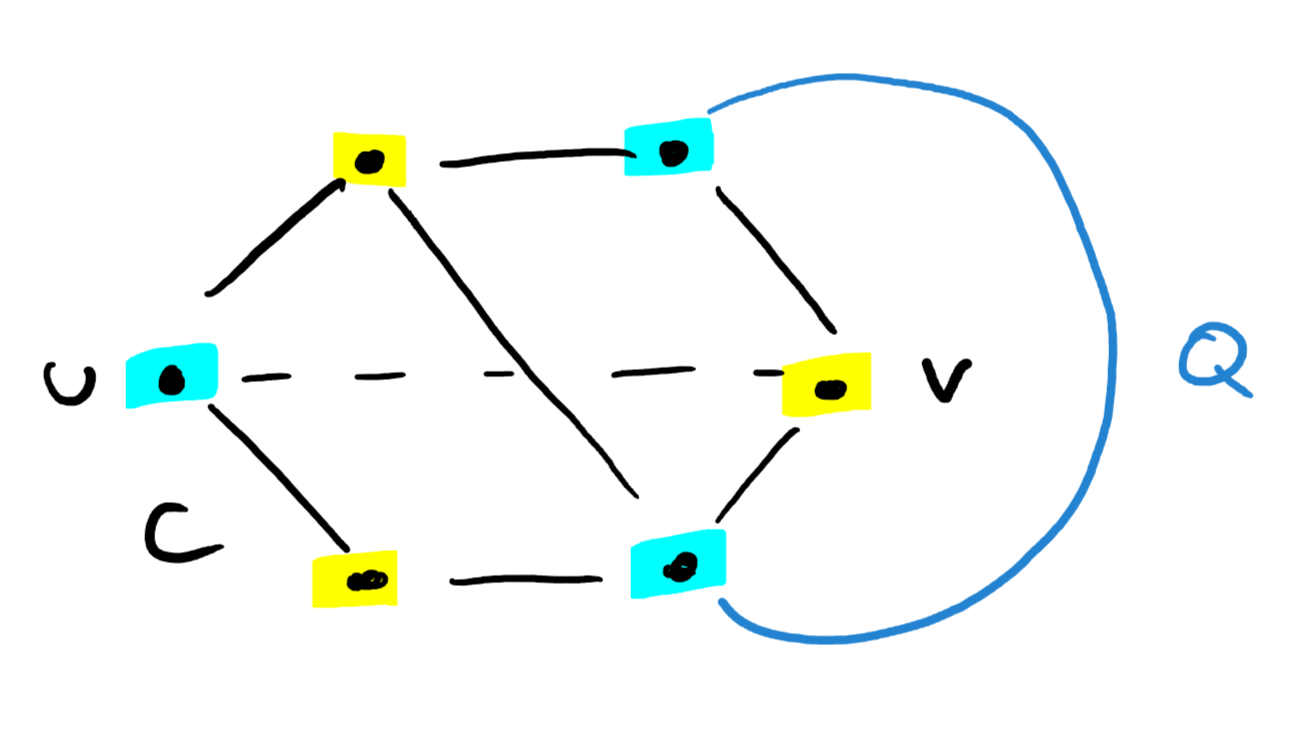
\includegraphics[width=\textwidth]{figures/kuratowski1.png}
            \subcaption{Gegenbeispiel 1}
            \label{fig:kuratowski-bsp1}
        \end{subfigure}
        \begin{subfigure}[c]{\w}
            \centering
            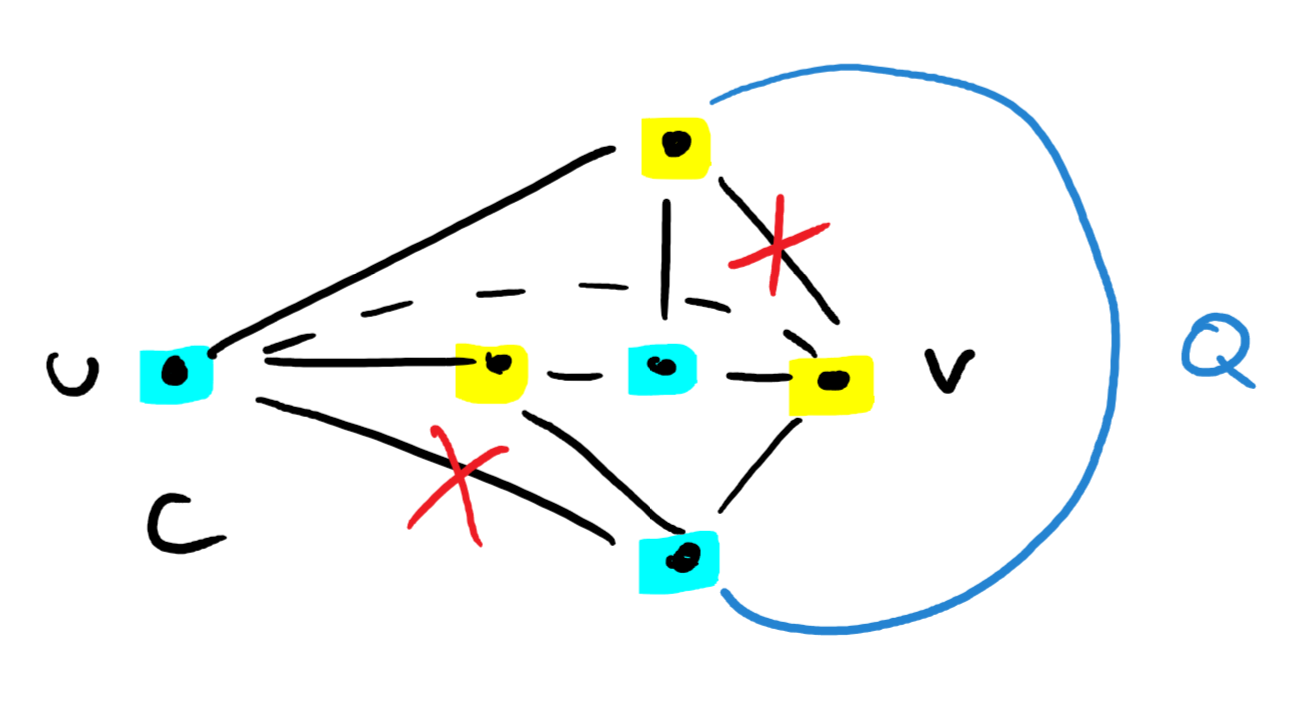
\includegraphics[width=\textwidth]{figures/kuratowski2.png}
            \subcaption{Gegenbeispiel 2}
            \label{fig:kuratowski-bsp2}
        \end{subfigure}
        \begin{subfigure}[c]{\w}
            \centering
            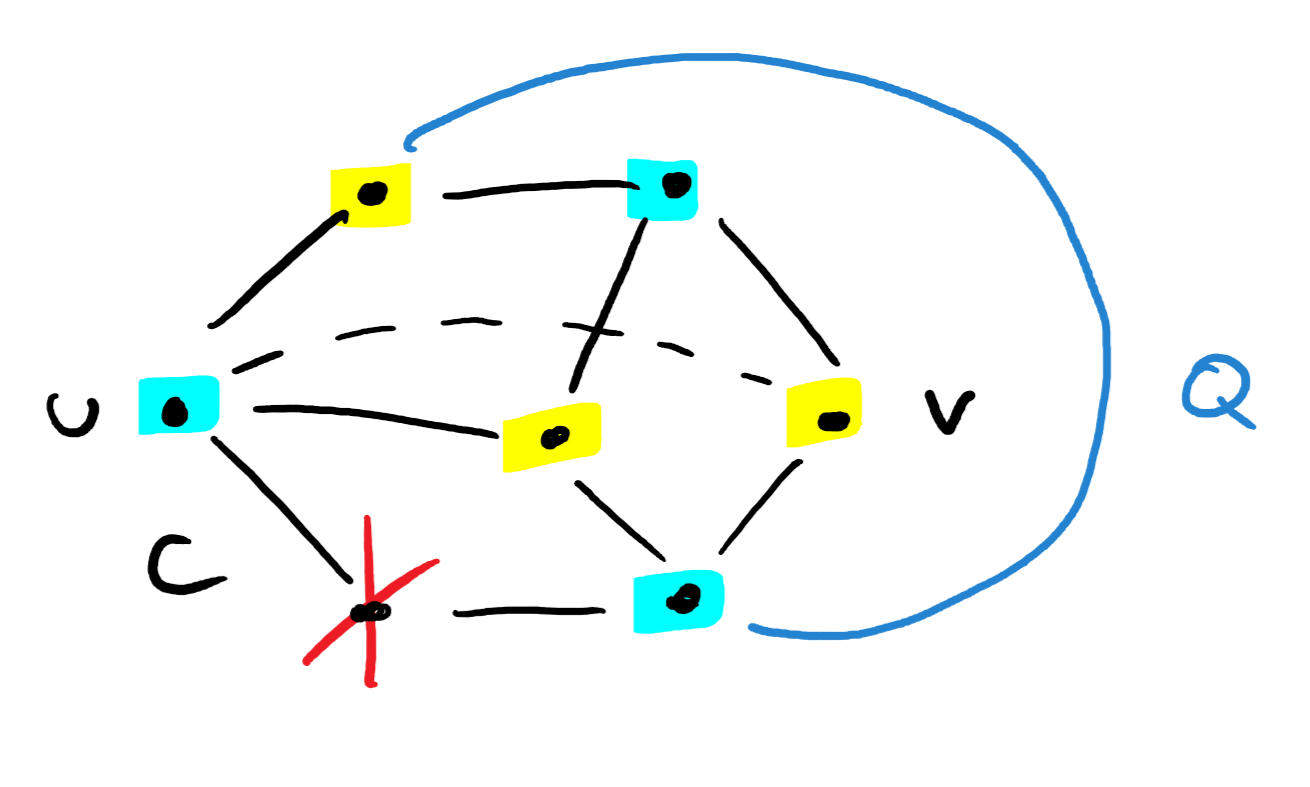
\includegraphics[width=\textwidth]{figures/kuratowski3.png}
            \subcaption{Gegenbeispiel 3}
            \label{fig:kuratowski-bsp3}
        \end{subfigure}
        \begin{subfigure}[c]{\w}
            \centering
            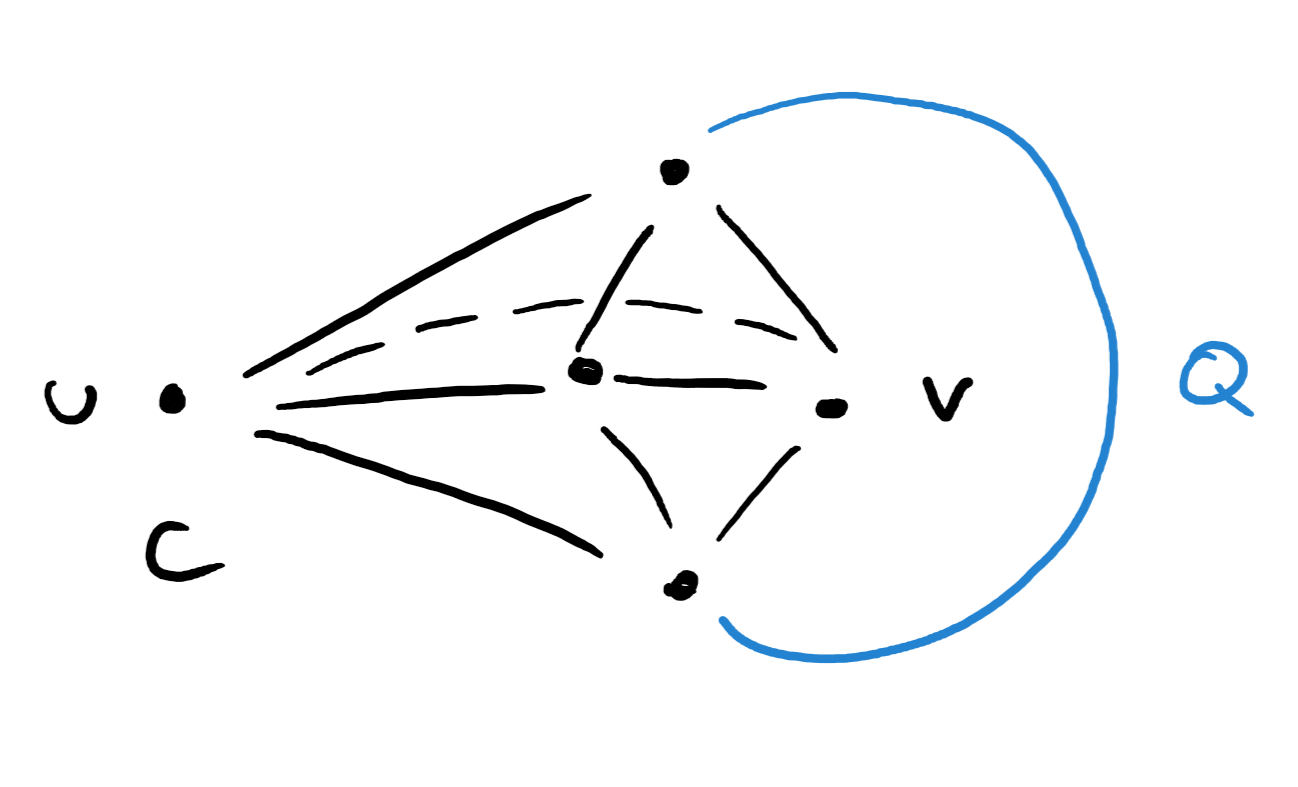
\includegraphics[width=\textwidth]{figures/kuratowski4.png}
            \subcaption{Gegenbeispiel 4}
            \label{fig:kuratowski-bsp4}
        \end{subfigure}
        \caption{Gegenbeispiele für den Beweis von Kuratowskis Theorem}
        \label{fig:kuratowski-bsp}
    \end{figure}
\end{proof}

\chapter{Graph-Färbung}

Im folgenden sei $ G = (V, E) $ ein fixierter Graph.

\begin{definition}[Coloring]
    Ein \textit{coloring} ist eine Funktion $ c : V \rightarrow \nats $ mit: wenn $ \{ u, v \} \in E $, dann $ c(u) \ne c(v) $.
\end{definition}

\begin{definition}[$ k $-Färbung]
    Ein Graph ist $ k $-färbbar, falls ein coloring $ c $ existiert mit $ |c(V)| \leq k $.
\end{definition}

\begin{definition}[Chromatische Zahl]
    Die chromatische Zahl $ \chi(G) $ eines Graphen ist definiert als das minimale $ k $, sodass $ G $ $ k $-färbbar ist.
\end{definition}

\begin{theorem}
    \label{thm:delta-coloring}
    Es gilt $ \chi(G) \leq \Delta(G) + 1 $.
\end{theorem}

\begin{proof}
    Färbe $ G $ greedy.
    Für $ v \in V $ mit $ v $ wurde noch nicht gefärbt, wähle die kleinste Farbe $ k \in \nats $, sodass kein Nachbar mit $ k $ gefärbt ist.
    Da jeder Knoten $ \Delta + 1 $ Nachbarn hat, ex. immer ein $ k \leq \Delta + 1 $, dass die Bedingung erfüllt.
\end{proof}

\begin{remark}
    Betrachte $ \{ v_1, \dots, v_{i - 1} \} \subseteq V $, die bereits greedy gefärbt wurden und Knoten $ v_i \in V $, der nun gefärbt werden soll.
    Für die Färbung von $ v_i $ werden maximal $ \deg_{G[\{ v_1, \dots, v_{i - 1} \}]}(v_i) + 1 $ Farben benötigt, nicht $ \deg(v_i) + 1 $.

    Der obige Algorithmus lässt sich also dahingehend verbessern, dass die Knoten nach Grad absteigend sortiert färbt.
\end{remark}

\begin{theorem}
    Für jeden Graph mit $ |E| = m $ gilt:
    \begin{equation*}
        \chi(G) \leq \frac{1}{2} + \sqrt{2m + \frac{1}{4}}
    \end{equation*}
\end{theorem}

\begin{proof}
    Sei $ c $ eine $ k $-Färbung mit $ k = \chi(G) $.
    Dann ex. mindestens eine Kante zwischen jeder Farbklasse.
    Andernfalls könnten zwei Klassen ohne Kante dieselbe Farbe nutzen.
    Also gilt:
    \begin{equation*}
        m \geq \frac{1}{2} \chi(G) (\chi(G) - 1)
    \end{equation*}
    Diese Gleichung kann entsprechend umgestellt werden.
\end{proof}

\begin{definition}[Clique]
    Eine Clique ist ein vollständiger verbundener (Teil-)Graph.
    $ K_\alpha $, $ \alpha \in \nats^+ $ bezeichnet den vollständigen Graphen mit $ \alpha $-vielen Knoten.
\end{definition}

\begin{proposition}
    Falls $ K_\alpha \subseteq G $, $ \alpha \in \nats^+ $, dann:
    \begin{equation*}
        \chi(G) \geq \alpha = \Delta(K_\alpha) + 1
    \end{equation*}
\end{proposition}

\begin{definition}[Odd-cycle]
    Sei $ C $ ein Kreis in $ G $.
    $ C $ ist ein \textit{odd-cycle}, falls $ |C| \mod 2 \ne 0 $.
\end{definition}

\begin{proposition}
    Gibt es einen odd-cycle in $ G $, gilt $ \chi(G) \geq 3 $.
\end{proposition}

\begin{lemma}
    \label{lem:min-deg-3-connected}
    Sei $ G $ 2-verbunden mit $ \delta(G) \geq 3 $.
    Falls $ G $ nicht vollständig ist, dann enthält $ G $ einen induzierten Pfad  $uvw $ auf 3 Knoten $ u, v, w \in V $, sodass $ G \setminus \{ u, w \} $ weiterhin verbunden ist.
\end{lemma}

\begin{proof}
    Da $ G $ verbunden aber nicht vollständig ist, ex. ein induzierter Pfad auf 3 Knoten.
    Falls $ G $ zusätzlich 3-verbunden ist, kann jeder solche Pfad für das Lemma gewählt werden.
    Es genügt daher, den Beweis nur für 2-verbundene Graphen zu führen.

    Sei $ \{ v, x\} \subseteq V $ ein cutset von $ G $.
    Dann ist $ G \setminus \{ v \} $ nicht 2-verbunden und hat zwei Blöcken $ B_1, B_2 $.
    Somit ex. zwei non-cut-vertices $ u \in B_1 $ und $ w \in B_2 $ adjazent zu $ v $.
    $ uvw $ ist der gesuchte Pfad.
\end{proof}

\begin{theorem}[Brooks' Theorem ('41)]
    Jeder Graph hat ein $ \Delta(G) $-coloring, außer:
    \begin{enumerate}
        \item \label{itm:brooks-vollst}
        $ G $ enthält einen vollst. Teilgraphen $ K_{\Delta(G) + 1} $ oder
        \item \label{itm:brooks-odd}
        $ \Delta(G) = 2 $ und $ G $ enthält einen odd-cycle.
    \end{enumerate}
\end{theorem}

\begin{proof}
    Nach Lov\'{a}sz ('75).

    Sei $ G $ verbunden.
    Es gelte weder \ref{itm:brooks-vollst} noch \ref{itm:brooks-odd}.
    Beweis per Fallunterscheidung:
    \begin{enumerate}
        \item \label{itm:deg-le-delta}
        Angenommen, $ G $  enthält einen Knoten $ v \in V $ mit $ \deg(v) < \Delta(G) $.

        Färbe $ G $ greedy mit Reihenfolge der Knoten sortiert nach Distanz zu $ v $, d.h. $ v $ wird zuletzt und die am weitesten von $ v $ entfernten Knoten zuerst gefärbt.
        Es gilt dann für $ u \in V $ mit $ u \ne v $, dass ein Nachbar $ w $ zu $ u $ ex., der noch nicht gefärbt wurde.
        Es werden also max. $ \Delta $ Farben gebraucht (vgl. Theorem \ref{thm:delta-coloring}).

        Insbesondere gilt $ \deg(v) < \Delta $ und damit wird $ v $ korrekt gefärbt.

        \item Angenommen, es sei $ v \in V $ ein cut vertex in $ G $, d.h. $ G $ nicht 2-verbunden.

        Für jede zusammenhängende Menge an Knoten $ V' \subseteq V $ von $ G \setminus \{ v \} $ gilt: $ G[V' \cup \{ v \}] $ kann mit $ \Delta(G) $-vielen Farben gefärbt werden, dafür $ G[V' \cup \{ v \}] $ Fall \ref{itm:deg-le-delta} gilt.

        Eine Färbung für $ G $ kann erzeugt werden, indem die Farbklassen von den Komponenten $ V' $ je so permutiert werden, dass $ v $ immer gleich gefärbt wird.

        \item Sei $ G $ $ \Delta(G) $-regulär, d.h. $ \forall v \in V: \deg(v) = \Delta(G) $, 2-verbunden und nicht vollständig.

        Sei $ uvw $ ein Pfad nach Lemma \ref{lem:min-deg-3-connected}.
        Färbe $ u $ und $ w $ mit Farbe 1.
        Färbe $ G \setminus \{ u , w \} $ greedy absteigend nach Distanz zu $ v $; hier trifft wieder Fall \ref{itm:deg-le-delta} zu.

        Schlussendlich kann auch $ v $ gefärbt werden, da $ u $ und $ w $ die gleiche Farbe nutzen.
    \end{enumerate}
\end{proof}

\begin{lemma}
    \label{lem:planar-degree}
    Sei $ G $ ein planarer Graph, dann gilt für den durchschnittlichen Knotengrad $ d(G) $: $ d(G) < 6 $.
\end{lemma}

\begin{proof}
    Es gilt $ d(G) = 2 \frac{|E|}{|V|} $.
    Mit $ |V| \geq 3 $, $ |E| \leq 3 |V| - 6 $ (cgl. Korollar \ref{cor:triangulation}).
    Dann gilt:
    \begin{align*}
        d(G) & \leq \frac{2 \cdot (3|V| - 6)}{|V|} \\
        &= 6 - \frac{12}{|V|} < 6
    \end{align*}
\end{proof}

\begin{theorem}
    Jeder planare Graph hat $ \chi(G) \leq 6 $.
\end{theorem}

\begin{proof}
    Beweis per Induktion über $ |V| $.
    \begin{description}
        \item[IS] Für $ |V| \leq 6 $ trivial.
        \item[IV] Es gelte, ein Graph mit $ n $ Knoten ist 6-färbbar.
        \item[IS] Sei $ G $ ein planarer Graph mit $ |V| = n + 1 $.

        Nach Lemma \ref{lem:planar-degree} existiert ein Knoten $ w \in V $ mit $ \deg(w) \leq 5 $.
        Sei $ G' = G \setminus \{ w \} $.
        Nach IV ist $ G' $ 6-färbbar.
        Sei $ c $ eine solche 6-Färbung.

        Da $ w $ nur 5 Nachbarn in $ G' $ hat, ex. eine Farbe $ k $ mit der $ w $ gefärbt werden kann, also ist auch $ G $ 6-färbbar.
    \end{description}
\end{proof}

\begin{theorem}
    Für jeden planaren Graphen $ G $ gilt $ \chi(G) \leq 5 $.
\end{theorem}

\begin{proof}
    Färbe zunächst alle Knoten $ v \in V $ mit $ \deg(v) < 5 $ rekursiv und greedy.
    Sei $ c $ diese Färbung.
    Es kann angenommen werden, dass $ G $ einen Knoten $ v $ mit $ \deg(v) = 5 $ enthält; andernfalls ist der Beweis trivial.

    Für $ v_1, v_2 \in V $ sei $ V_{v_1, v_2} = \{ v \in V \mid c(v) \in \{ c(v_1), c(v_2) \} \} $ und $ V^*_{v_1, v_2} = \{ v \in V \mid $ es ex. Pfad von $ x $ nach $ v $ in $ V_{x, y} \} $.

    Betrachte $ x, y \in V $ mit $ c(x) \ne c(y) $.
    Fallunterscheidung:
    \begin{enumerate}
        \item \label{itm:case-color-xy}
        Angenommen, es ex. kein Pfad $ P $ in $ V_{x,y} $ von $ y $ nach $ x $.
        Dann gilt $ V^*_{x,y} \cap V^*_{y,x} = \emptyset $.

        Dann definiere neue Färbung $ c' $, die die Farben in $ V^*_{x, y} $ tauscht:
        \begin{equation*}
            c'(s) = \begin{cases}
                c(s), & s \notin V^*_{x, y}, \\
                c(x), & s \in V^*_{x,y}, c(s) \ne c(x) \\
                c(y), & s \in V^*{x,y}, c(s) = c(x)
            \end{cases}
        \end{equation*}

        Somit kann in $ v $ in $ c' $ auf $ c(x) $ gesetzt werden.

        \item Angenommen, es ex. ein Pfad $ P $ in $ V_{x,y} $ von $ x $ nach $ y $.

        Betrachte Nachbarn $ t, z \in V $ von $ v $; dargestellt in Abbildung \ref{fig:5-colorable}.
        Es gilt: $ V_{t,z} \cap V_{x,y} = \emptyset $.

        Dann muss gelten, dass $ V^*_{t,z} \cap V^*_{z,t} = \emptyset $ oder Widerspruch zu $ G $ ist planar.
        Somit lassen sich $ t $ und $ z $ nach Fall \ref{itm:case-color-xy} umfärben.
    \end{enumerate}

    \begin{figure}
        \centering
        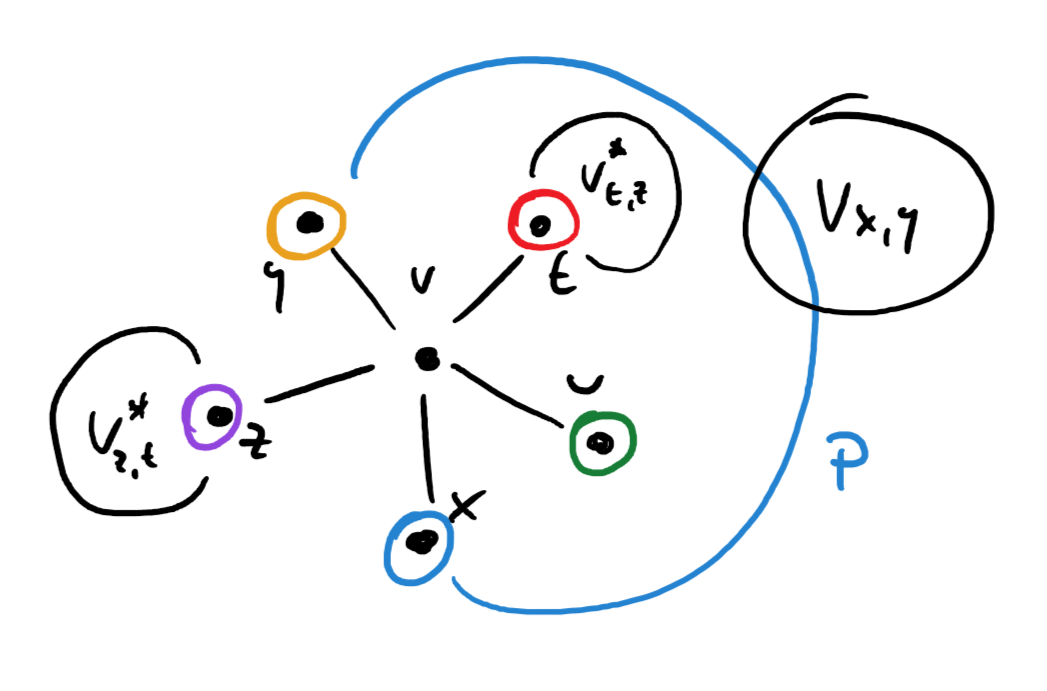
\includegraphics[width=0.45\textwidth]{figures/5-colorable.png}
        \caption{Beweis 5-Farbensatz Veranschaulichung}
        \label{fig:5-colorable}
    \end{figure}
\end{proof}

\chapter{Zufällige Graphen}

Im folgenden sei $ \mathcal{G} $ die Menge aller Graphen und $ G = (V, E) $ mit $ V = \{ 0, \dots, n - 1 \} $ ein fixierter Graph.

\begin{definition}
    Sei $ V $ eine Menge von Knoten.
    \begin{equation*}
        [V]^2 = \{ \{ v_1, v_2 \} \mid v_1, v_2 \in V \}
    \end{equation*}
\end{definition}

\begin{definition}[Elementares Ereignis]
    Sei die Menge an Knoten $ V $ fixiert und $ G_0 $ ein fixierter Graph mit den Knoten $ V $ und $ m $ Kanten.
    Dann ist $ \{ G_0 \} $ das sog. \textit{elementare Ereignis}.

    Sei $ p \in [0, 1]$ die Wahrscheinlichkeit, eine Kante $ e \in E \subseteq [V]^2 $ zu auszuwählen.
    Dann gilt:
    \begin{equation*}
        P(\{ G_0 \}) = p^m \cdot (1 - p)^{\binom{n}{2} - m}
    \end{equation*}
\end{definition}

Im folgenden gelte $ q = 1 - p $.

\begin{definition}
    Sei $ e \in [V]^2 $.
    Definiere den Wahrscheinlichkeitsraum $ \Omega_e = \{ 0_e, 1_e \} $ mit:
    \begin{itemize}
        \item $ P(\{ 1_e \}) = p $ und
        \item $ P(\{ 0_e \}) = 1 - p = q $.
    \end{itemize}
\end{definition}

\begin{definition}
    $ \mathcal{G} = \mathcal{G}(n, p) $ bezeichne den Produktraum über
    \begin{align*}
        \Omega &= \prod_{e \in [V]^2} \Omega_e \\
        &= \{ 0_0, 1_0 \} \times \{ 0_1, 1_1 \} \times \dots
    \end{align*}

    Interpretiere dabei $ \omega \in \Omega $ als Funktion, d.h. $ \omega : [V]^2 \rightarrow \{ 0, 1 \} $.
    $ \omega $ korrespondiert zu dem Graphen $ G_\omega = (V, \{ e \mid \omega(e) = 1 \}) $.
\end{definition}

\begin{remark}
    Das Ziehen einer Menge von Graphen über $ n $ Knoten mit der Kanten-Wahrscheinlichkeit $ p $ ist ein Ereignis in $ \mathcal{G}(n, p) $.

    Insbesondere für $ e \in [V]^2 $ ist $ A_e = \{ \omega \in \Omega \mid \omega(e) = 1 \} $ ein Ereignis.
\end{remark}

\begin{proposition}
    Für $ e \in [V]^2 $ ist $ A_e $ unabhängig.
\end{proposition}

\begin{proof}
    Es ist offensichtlich, dass $ A_e = \{ 1_e \} \times \prod_{e' \in [V]^2, e' \ne e} \Omega_{e'} $.
    Es gilt:
    \begin{align*}
        P(A_e) &= p \cdot \prod_{e' \in [V]^2, e' \ne e} 1 \\
        &= p
    \end{align*}
\end{proof}

\begin{remark}
    Ähnliches gilt für $ \{ e_1, \dots, e_k \} \subseteq [V]^2 $.
    Dann ist $ P(A_{\{ e_1, \dots, e_k \}}) = P(A_{e_1} \cap \dots \cap A_{e_k}) = p^k $.
\end{remark}

\begin{proposition}
    Sei $ H = (V_H, E_H)$ ein fixierter Graph mit $ |V_H| \leq |V| $ und $ |E_H| \leq |E| $.

    Für die Wahrscheinlichkeit $ P(H \subseteq G) $, dass $ G $ zufällig gezogen wird mit $ H \subseteq G $, gilt: $ P(H \subseteq G) = p^{|E_H|} $.

    Für die Wahrscheinlichkeit $ P(H = G[V_H]) $, dass $ G $ zufällig gezogen wird mit $ H = G[V_H] $, gilt $ P(H = G[V_H]) = p^{|E_H|} \cdot (1 - p)^{\binom{|V_H|}{2} - |E_H|} $.
\end{proposition}

\begin{definition}[Unabhängige Mengen]
    Eine Menge $ M \subseteq V $ ist unabhängig, falls $ \forall v_1, v_2 \in M: \{ v_1, v_2 \} \notin E $.
\end{definition}

\begin{definition}[Independence Number]
    Die independence number $ \alpha(G) $ ist die maximale Anzahl unabhängiger Knoten, d.h. die Kardinalität der größten unabhängigen Menge in $ G $.
\end{definition}

\begin{lemma}
    \label{lem:independent-prob}
    Für alle $ n, k \in \nats $ mit $ 2 \leq k \leq n $ gilt für die Wahrscheinlichkeit $ P(\alpha(G) \geq k) $, dass ein zufälliger Graph $ G $ aus $ \mathcal{G}(n, p) $ mindestens eine Menge von $ k $ unabhängigen Knoten besitzt:
    \begin{equation*}
        P(\alpha(G) \geq k) \leq \underbrace{\binom{n}{k}}_{\text{Anzahl Teilmengen}} \cdot \underbrace{(1 - p)^{\binom{k}{2}}}_{\text{Teilmenge ist unabhängig}}
    \end{equation*}
\end{lemma}

\begin{lemma}
    Mit $ k \leq n $ gilt für die Wahrscheinlichkeit $ P(K_k \subseteq G) $, dass ein zufälliger Graph $ G $ $ K_k $ als Teilgraphen hat, d.h., dass die Anzahl Knoten in der größten Clique von $ G $ $ cli(G) $ größer gleich $ k $ ist:
    \begin{equation*}
        P(K_k \subseteq G) = P(cli(G) \geq k) \leq \binom{n}{k} \cdot p^{\binom{k}{2}}
    \end{equation*}
\end{lemma}

\begin{lemma}
    Für $ k \leq n $ gilt: Falls $ P(\alpha(G) \geq k) + P(cli(G) \geq k) < 1 $, dann gibt es Graphen $ G $ ohne entsprechende Clique \textit{und} unabhängige Menge über $ V $.
\end{lemma}

\begin{definition}
    Sei $ X_k : \mathcal{G}(n, p) \rightarrow \nats $ die Zufallsvariable, die einem Graphen über $ V $ die Anzahl an $ k $-Kreisen zuweist.
\end{definition}

\begin{proposition}
    Sei $ \mathcal{C}_k $ die Menge aller $ k $-Kreise in $ G $ modulo Isomorphie.
    Sei:
    \begin{equation*}
        (n)_k = \prod_{0 \leq i \leq k - 1} (n - i) = n \cdot (n - 1) \cdot \dots \cdot (n - k + 1) = \frac{n!}{(n - k)!}
    \end{equation*}
    $ (n)_k $ ist die Anzahl an Möglichkeiten, $ k $ unterschiedliche Knoten in $ V $ zu wählen.
    Des Weiteren gibt es zu jedem $ k $-langen Kreis $ 2k $-viele Isomorphie Kreise.

    Es gilt somit:
    \begin{equation*}
        |\mathcal{C}_k| = \frac{(n)_k}{2k}
    \end{equation*}
\end{proposition}

\begin{proposition}
    Der Erwartungswert von $ X_k $ ist:
    \begin{equation*}
        E(X_k) = \frac{(n)_k}{2k} \cdot p^k
    \end{equation*}
\end{proposition}

\section{Färben zufälliger Graphen}

\begin{proposition}
    Sei $ p \in (0, 1) $ und $ \epsilon > 0 $.
    Dann gilt, für fast jeden Graph $ G \in \mathcal{G}(n, p) $:
    \begin{equation*}
        \chi(G) > \frac{\log(\frac{1}{q})}{2 + \epsilon} \cdot \frac{n}{\log(n)}
    \end{equation*}
\end{proposition}

\begin{proof}
    Für $ 2 \leq k \leq n $ gilt nach Lemma \ref{lem:independent-prob}:
    \begin{align*}
        P(\alpha(G) \geq k) & \leq \binom{n}{k} q^{\binom{k}{2}} \\
        & \leq n^k \cdot q^{\binom{k}{2}} \\
        &= q^{k \cdot \frac{\log(n)}{\log(q)} + \frac{1}{2}k(k - 1)} \\
        &= q^{\frac{k}{2} \cdot (-2 \frac{\log(n)}{\log(q^{-1})} + k - 1)}
    \end{align*}

    Für $ k := 2 + \epsilon \frac{\log(n)}{\log(q^{-1})} $ gilt $ \frac{k}{2} \cdot (-2 \frac{\log(n)}{\log(q^{-1})} + k - 1) $ geht gegen $ \infty $ für $ n \rightarrow \infty $.

    Somit gilt für fast jeden Graphen $ G \in \mathcal{G}(n, p) $: In irgendeiner Färbung von $ G $ gibt es keine $ k $ Knoten derselben Farbe.

    Somit sind mehr als $ \frac{n}{k} = \frac{\log(q^{-1})}{2 + \epsilon} \cdot \frac{n}{\log(n)} $ Farben nötig.
\end{proof}

\section{Eigenschaften fast aller Graphen}

\begin{proposition}
    Für $ p \in (0, 1) $ und einen fixen Graph $ H $ gilt, fast jeder Graph $ G \in \mathcal{G}(n, p) $ enthält einen induzierten Graph $ H $.
\end{proposition}

\begin{proof}
    Sei $ H $ gegeben und $ k = |H| $.
    Wenn $ n = |V| \geq k $ und $ U \subseteq V $ mit $ |U| = k $, dann ist $ H $ isomorph zu $ G[U] $ mit Wahrscheinlichkeit $ r > 0 $.
    $ r $ hängt von $ p $, aber nicht $ n $ ab, da $ U $ fixiert.
    $ G $ besteht aus $ \lfloor \frac{n}{k} \rfloor $ vielen disjunkten Mengen $ U $.

    Die Wahrscheinlichkeit, dass keiner dieser induzierten Graphen $ G[U_i] $ isomorph zu $ H $ ist, ist $ (1 - r)^{\lfloor \frac{n}{k} \rfloor} $.
    Diese Ereignisse sind unabhängig, da $ U_i $ paarweise disjunkt.

    Es gilt:
    \begin{equation*}
        P(H \not \subseteq G[U_i], i \in [1, \lfloor \frac{n}{k} \rfloor]) \leq (1 - r)^{\frac{n}{k}} \xrightarrow[n \to \infty]{} 0
    \end{equation*}
\end{proof}

\chapter{Graph Produkte}

\begin{definition}[Produkt]
    Seien $ G, H $ Graphen.
    Definiere $ \boxop $ Operator:
    \begin{itemize}
        \item $ V(G \boxop H) = V(G) \times V(H) $
        \item $ \{ (x, y), (u, v) \} \in E(G \boxop H) $ gdw. \begin{enumerate}
            \item $ \{ x, u \} \in E(G) $ und $ y = v $ oder
            \item $ \{ y, v \} \in E(H) $ und $ x = u $.
        \end{enumerate}
    \end{itemize}
\end{definition}

\begin{proposition}
    Für $ \boxop $ gilt:
    \begin{itemize}
        \item Ein \textit{neutrales Element} existiert: $ G \boxop K_1 \cong G $
        \item Assoziativität: $ (G \boxop H) \boxop I \cong G \boxop (H \boxop I) $
        \item Kommutativität: $ G \boxop H \cong H \boxop G $
    \end{itemize}
\end{proposition}

\begin{theorem}
    Sei $ G $ ein Graph, dann gibt es eine eindeutige Multi-Menge von Graphen $ G_i \neq K_i $ mit:
    \begin{enumerate}
        \item $ G = \boxop^k_{i = 1} G_i $ und
        \item $ G_i $ ist prim, d.h., wenn $ G_i = H_1 \boxop H_2 $, dann $ H_1 = K_1 $ oder $ H_2 = K_1 $.
    \end{enumerate}
\end{theorem}

\begin{remark}
    Eine Primfaktorzerlegung bzgl. des Graph-Produkts lässt sich in Linearzeit berechnen.
\end{remark}

\begin{definition}[Hamming-Graph]
    $ G $ ist ein \textit{Hamming-Graph}, falls er sich für ein $ n \in \nats $ darstellen lässt als ein Produkt vollständig verbundener $ n $ Graphen:
    \begin{equation*}
        \boxop^k_{i = 1} K_n
    \end{equation*}
\end{definition}

\begin{remark}
    Bspw. sind alle $ n $-dimensionalen Hyperwürfel ein Hamming-Graph auf Basis von $ K_2 $.

    Ein Hamming-Graph lässt einen die Hamming-Distanz von Wörter über einem Alphabet der Größe $ n $ direkt aus der Distanz im Graphen ablesen.
    Jeder Knoten im $ K_n $ Graph repräsentiert einen Buchstaben des Wortes, ein Tupel-Knoten im $ K_n^k $-Hamming-Graphen ein Wort.
\end{remark}

\begin{definition}[Direktes Produkt]
    Seien $ G, H $ Graphen.
    Definiere das \textit{direkte Produkt} $ G \times H $ als:
    \begin{itemize}
        \item $ V(G \times H) = V(G) \times V(H) $ und
        \item $ \{ (x, y), (u, v) \} \in E(G \times H) $ gdw. $ \{ x, u\} \in E(G) \land \{ y, v \} \in E(H) $.
    \end{itemize}
\end{definition}

\begin{definition}[Starkes Produkt]
    Seien $ G, H $ Graphen.
    Definiere das \textit{starke Produkt} $ G \boxtimes H $ als:
    \begin{itemize}
        \item $ V(G \boxtimes H) = V(G) \times V(H) $ und
        \item $ E(G \boxtimes H) = E(G \times H) \cup E(G \boxop H) $.
    \end{itemize}
\end{definition}

\begin{proposition}
    Für alle $ p, q \in \nats $ gilt:
    \begin{equation*}
        K_p \boxtimes K_q \cong K_{(p \cdot q)}
    \end{equation*}

    Somit ist $ K_n $ Prim-Graph der vollständigen Graphen bzgl. des starken Produkts gdw. $ n $ ist eine Primzahl.
\end{proposition}

\begin{definition}[Modulares Produkt]
    Seien $ G, H $ Graphen.
    Definiere das \textit{modulare Produkt} $ G * H $ als:
    \begin{itemize}
        \item $ V(G * H) = V(G) \times V(H) $ und
        \item $ \{ (u, x), (v, y) \} \in E(G * H) $ gdw.
        \begin{enumerate}
            \item $ \{ u, v \} \in E(G) $ und $ \{ x, y \} \in E(H) $ oder
            \item $ \{ u, v \} \notin E(G) $ und $ \{ x, y \} \notin E(H) $.
        \end{enumerate}
    \end{itemize}
\end{definition}

\begin{remark}
    Jeder vollständige Teilgraph von $ G * H $ entspricht einem gemeinsamen induzierten Teilgraph von $ G $ und $ H $.
\end{remark}

\chapter{Co-Graphen}

\begin{definition}[Disjunkte Vereinigung]
    Seien $ G = (V_G, E_G), H = (V_H, E_H) $ Graphen.
    Definiere die \textit{disjunkte Vereinigung} $ \discup $ zweier Graphen als:
    \begin{equation*}
        G \discup H = \big(V_G \discup V_H, E_G \discup E_H\big)
    \end{equation*}
\end{definition}

\begin{definition}[Join]
    Seien $ G = (V_G, E_G), H = (V_H, E_H) $ Graphen.
    Definiere den \textit{Join} $ \join $ zweier Graphen als:
    \begin{align*}
        G \join H = (& V_G \discup V_H, \\
        & E_G \discup E_H \cup \{ \{ x, y \} \mid x \in V_G, y \in V_H \})
    \end{align*}
\end{definition}

\begin{definition}[Komplement]
    Definiere das \textit{Komplement} $ \overline{\circ} $ eines Graphen als:
    \begin{equation*}
        \overline{G} = (V, (V \times V) \setminus E)
    \end{equation*}
\end{definition}

\begin{definition}[Co-Graphen]
    Die Menge der Co-Graphen $ \mathcal{C} $ sei induktiv definiert als die kleinste Menge, für die gilt:
    \begin{enumerate}
        \item $ K_1 \in \mathcal{C} $;
        \item wenn $ G, H \in \mathcal{C} $, dann \begin{enumerate}
            \item $ G \discup H \in \mathcal{C} $ und
            \item $ G \join H \in \mathcal{C} $.
        \end{enumerate}
    \end{enumerate}
\end{definition}

\begin{proposition}
    $ G $ ist ein Co-Graph gdw. $ \overline{G} $ ist ein Co-Graph.
\end{proposition}

\begin{definition}[Test auf Co-Graphen]~\par
    \begin{enumerate}
        \item \label{itm:co-alg-rec}
        Bilde zu jeder Zusammenhangskomponente von $ G $ das Komplement.
        \item Sind nicht alle nun bestehenden Zusammenhangskomponente isomorph zu $ K_1 $, gehe zu \ref{itm:co-alg-rec}.
    \end{enumerate}

    Dieser Algorithmus zerlegt einen Graphen sukzessive in einem Baum von Zusammenhangskomponenten, den sog. \textit{Co-Tree}.
\end{definition}

\begin{proposition}[Charakterisierung von Co-Graphen]
    Sei $ P_4 = (\{ 0, \dots, 3 \}, \{ \{ i, i + 1\} \mid 0 \leq i < 3 \}) $.
    $ G $ ist ein Co-Graph gdw. er enthält keinen $ P_4 $.
\end{proposition}

\begin{proposition}
    $ P_4 $ ist 2-färbbar.
\end{proposition}

\begin{definition}[Grundy-Zahl]
    Die \textit{Grundy-Zahl} eines Graphen $ G $ ist die Zahl der Farben, die bei einer Greedy-Färbung benötigt wird.
\end{definition}

\begin{definition}[Wohl-färbbar]
    Ein Graph $ G $ ist \textit{wohl-färbbar}, falls seine Grundy-Zahl gleich $ \chi(G) $.
\end{definition}

\begin{proposition}
    $ G $ ist wohl-färbbar gdw. $ G $ ist ein Co-Graph.
\end{proposition}

\begin{proposition}
    Jeder induzierte Teilgraph eines Co-Graphen ist wieder ein Co-Graph.
\end{proposition}


\end{document}
